\section{Introduction}
\subsection{Definitions and presentation}
  \begin{frame}
    \frametitle{Definitions}
      \begin{itemize}
        \item \textbf{Network:} an \textbf{interconnected} group or system\pause
        \item \textbf{Internet:} world wide \textbf{interconnected system of network\emph{s}} \color{blue}\href{http://tools.ietf.org/html/rfc791}{RFC791 (1981)}\color{black}\pause
        \item \textbf{IP:} Internet \textbf{Protocol} that provides the functions necessary to deliver a package of bits from a source to a destination over a network\pause
        \item \textbf{(world wide) Web:} \textbf{network} consisting of a collection of Internet websites using HTTP\pause
        \item \textbf{HTTP:} Hypertext Transfer Protocol \textbf{Protocol}, application-level protocol for distributed, collaborative, hypermedia information systems \color{blue}\href{http://tools.ietf.org/html/draft-ietf-httpbis-http2-14}{draft HTTP2 (July 2014)} \color{black}
      \end{itemize}
  \end{frame}
  \begin{frame}
    \frametitle{Definitions}
      \begin{itemize}
        \item \textbf{Router:} network \textbf{hardware} providing routing services\pause
        \item \textbf{Routing:} \textbf{algorithm processed} to decide where to forward a packet\pause
        \item \textbf{Forwarding:} \textbf{\emph{action}} of moving a packet from an NIC to another\pause
        \item \textbf{NIC:} Network Interface Card
        \item \textbf{Switch (hub):} network \textbf{hardware} that connect systems together using packet switching\pause
        \item \textbf{Packet switching:} forward-like method regardless of the content (destination-based)\pause
      \end{itemize}
  \end{frame}
  \begin{frame}
    \frametitle{Definitions}
      \begin{itemize}
        \item \textbf{Computer (network):} any entity that can send/receive packets from a network through a NIC\pause
        \item \textbf{Client:} \textbf{computer} able to send requests to a server\pause
        \item \textbf{Request:} \textbf{application message} destined for a server (\emph{order})\pause
        \item \textbf{Server:} \textbf{computer} able to respond a client's requests\pause
        \item \textbf{Request:} \textbf{application message} destined for a client (\emph{result})\pause
        \item \textbf{Fat client:} \textbf{application} where most functions are processed by the client itself\pause
        \item \textbf{Thin client:} \textbf{application} where most functions are carried out on a central server
      \end{itemize}
  \end{frame}

\subsection{HTTP request/response example}
\begin{frame}
    \frametitle{Example}
      Enter \color{blue}\href{http://getbootstrap.com}{getbootstrap.com} \color{black} in your browser\pause
      \begin{figure}
	  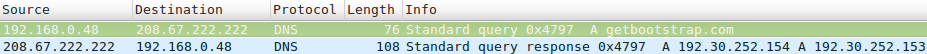
\includegraphics[width=11.5cm]{./imgs/dns-req.png}
	\caption{DNS request/response}
      \end{figure}
      \pause
      \begin{figure}
	  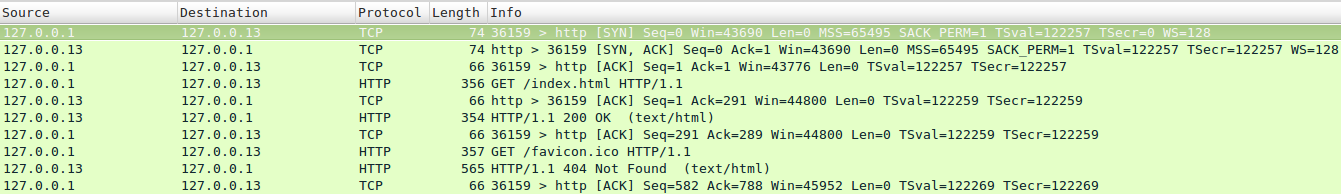
\includegraphics[width=13cm]{./imgs/http-req.png}
	\caption{HTTP request/response}
      \end{figure}
  \end{frame}
    \begin{frame}
    \frametitle{How does messages reach destination ?}
      \begin{figure}
	  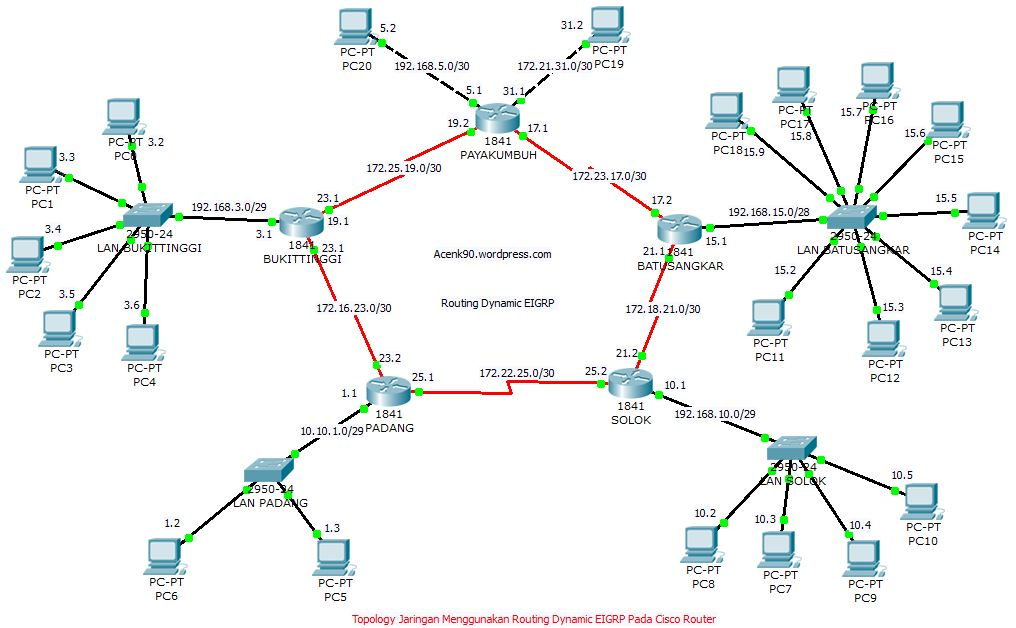
\includegraphics[width=9.5cm]{./imgs/routing.jpg}
	\caption{\color{blue}\href{http://acenk90.files.wordpress.com}{acenk90.files.wordpress.com}}
	\label{fig:routing}
      \end{figure}
  \end{frame}


\subsection{Network classification}
  \begin{frame}
    \frametitle{What kind of networks is it ?}
      \begin{itemize}
        \item \textbf{PAN:} Personal Area Networks are used for communication among various devices, such as telephones, personal digital assistants, fax machines, and printers, that are located close to a single user.
        \item \textbf{(W)LAN:} (Wireless) Local Area Networks cover a small physical area, like a home, office, or a small group of buildings, such as a school or airport.
        \item \textbf{MAN:} Metropolitan Area Networks are very large networks that cover an entire city.
        \item \textbf{WAN:} Wide Area Networks cover a broad area, like communication links that cross metropolitan, regional, or national boundaries. The Internet is the best example of a WAN.
      \end{itemize}
  \end{frame}


\subsection{Models overview (OSI and TCP/IP)}
  \begin{frame}
    \frametitle{How does it work ?}
    %http://homepages.uel.ac.uk/u0313643/photo.htm
  \end{frame}